% TODO: Consider using modern I2C terms: "controller" & "peripheral"/"target" vs. "master" & "slave"
% Note: remove `openany` for printed version
\documentclass[12pt,a4paper,openany,dutch,english]{extbook}
\usepackage[a4paper,includeheadfoot,margin=2.50cm]{geometry}


% By default, LaTeX tries to stretch whitespace between paragraphs on a page in order to reduce whitespace at the end of the page. This sometimes gives ugly results. The following command disables that stretching.
\raggedbottom % Don't reduce whitespace at the end of a page.

\renewcommand{\baselinestretch}{1.2}  % stretch horizontal space between everything by 20%


\usepackage[hyphens]{url} % Break line on hyphens in long urls
\usepackage{graphicx}
\graphicspath{{images/}}
\usepackage{pdfpages}
\usepackage{enumitem}
\usepackage{float}
\usepackage{caption}
\usepackage{subcaption}
\usepackage[toc,page]{appendix}
\usepackage{fontspec}

% Don't indent table of contents, list of figures, and list of tables
\usepackage{tocloft}
\setlength{\cftsecindent}{0pt}    % Remove indent for \section in Table of Contents
\setlength{\cftsubsecindent}{0pt} % Remove indent for \subsection in Table of Contents
\setlength{\cftfigindent}{0pt}    % remove indentation from figures in List of Figures
\setlength{\cfttabindent}{0pt}    % remove indentation from tables in List of Tables

\usepackage{parskip} % Add space between two paragraphs and don't indent the first line of the paragraph

% To generate fake lorem ipsum text
\usepackage{lipsum}


% \setmainfont{Arial}
%
% UGent style guide
% zet onderstaande lijnen uit commentaar om het font in te stellen
\setmainfont[
	Path=fonts/,
	BoldFont      =UGentPannoText-SemiBold.ttf,
	ItalicFont    =UGentPannoText-Normal.ttf,
	ItalicFeatures={FakeSlant=0.3},
	BoldItalicFont=UGentPannoText-SemiBold.ttf,
   BoldItalicFeatures={FakeSlant=0.3},
]{UGentPannoText-Normal.ttf}

\urlstyle{same} % Also use the default font for URLs


% If you want left justified text, uncomment the line below.
% \usepackage[document]{ragged2e} % Left justify all text

% Style Chapter titles so they have the chapter number in grey.
\usepackage{color}
\definecolor{chaptergrey}{rgb}{0.5,0.5,0.5}
\usepackage[explicit, pagestyles]{titlesec}
\titleformat{\chapter}[display]{\bfseries}{\color{chaptergrey}\fontfamily{lmr}\fontsize{80pt}{100pt}\selectfont\thechapter}{0pt}{\Huge #1}
\titlespacing*{\chapter}{0pt}{-80pt}{30pt}


% Header showing chapter number and title and footer showing page number
\newpagestyle{fancy}{%
  \sethead{} % left
          {} % center
          {\Large\thechapter~~\chaptertitle} %right
  \setfoot{} % left
          {\thepage} % center
          {} %right
  \setheadrule{0pt}
}
\pagestyle{fancy}

% Header showing chapter title and footer showing page number
\newpagestyle{numberless}{%
  \sethead{} % left
          {} % center
          {\Large\chaptertitle} %right
  \setfoot{} % left
          {\thepage} % center
          {} %right
  \setheadrule{0pt}
}

% We use the package `minted` for modern code highlighting.
\usepackage[newfloat,chapter]{minted}
\SetupFloatingEnvironment{listing}{name=Code Fragment, listname=List of Code Fragments}
\usemintedstyle{pastie} % for other highlighting color schemes, see https://www.overleaf.com/learn/latex/Code_Highlighting_with_minted#Reference_guide

\PassOptionsToPackage{hyphens}{url}
\usepackage{hyperref}
\usepackage{url}

\usepackage[numbers]{natbib}       % For bibliography; use numeric citations
\bibliographystyle{IEEEtran}
\usepackage[nottoc]{tocbibind}     % Put Bibliography in ToC

%
% Defines \checkmark to draw a checkmark
%
\usepackage{tikz}
\def\checkmark{\tikz\fill[scale=0.4](0,.35) -- (.25,0) -- (1,.7) -- (.25,.15) -- cycle;}

%
% For tables
%
\usepackage{booktabs}
\usepackage{array}
\usepackage{ragged2e}  % for '\RaggedRight' macro (allows hyphenation)
\newcolumntype{L}[1]{>{\raggedright\let\newline\\\arraybackslash\hspace{0pt}}m{#1}}
\newcolumntype{C}[1]{>{\centering\let\newline\\\arraybackslash\hspace{0pt}}m{#1}}
\newcolumntype{R}[1]{>{\raggedleft\let\newline\\\arraybackslash\hspace{0pt}}m{#1}}

%
% Support for splitting Dutch words correctly
%
\usepackage{polyglossia}
\setmainlanguage{english}

% Fix error "Package hyperref Warning: The anchor of a bookmark and its parent's must not be the same. Added a new anchor on ..."
\newcommand{\sectionbreak}{\phantomsection}


\usepackage[toc,acronym]{glossaries}  % for list of acronyms
\makeglossaries                       % start internal list of acronyms

% TODO: Bepalen of ik dit wel wil. Text dan met iets meer "spaties" tussen woorden, maar vermijdt wel ongemakkelijke woordafbrekingen.
\hyphenpenalty=5000
\tolerance=1000

%
% Set the title and your name
%
%%%%%%%%%%%%%%%%%%%%%%%%%%%%%%%%%%%%%%%%%%%%%%%%%%%%%%%%%%%%%%%%%%%%%%
%
% Add the specific info for your thesis
%
%%%%%%%%%%%%%%%%%%%%%%%%%%%%%%%%%%%%%%%%%%%%%%%%%%%%%%%%%%%%%%%%%%%%%%

\title{Collaborative Compositions: Facilitating Service Orchestration from Cloud to Edge}
\author{Merlijn Sebrechts}







%%%%%%%%%%%%%%%%%%%%%%%%%%%%%%%%%%%%%%%%%%%%%%%%%%%%%
% Add all the acronyms you use in your thesis here. %
% These will be added to the List of Acronyms       %
%%%%%%%%%%%%%%%%%%%%%%%%%%%%%%%%%%%%%%%%%%%%%%%%%%%%%


\newacronym{IP}{IP}{Internet Protocol}
\newacronym{CPU}{CPU}{Central Processing Unit}
\newacronym{vCPU}{vCPU}{Virtual Central Processing Unit}
\newacronym{RAM}{RAM}{Random Access Memory}
\newacronym{TCP}{TCP}{Transmission Control Protocol}
\newacronym{VM}{VM}{Virtual Machine}
\newacronym{IT}{IT}{Information Technology}
\newacronym{API}{API}{Application Programming Interface}
\newacronym{UI}{UI}{User Interface}
\newacronym{GUI}{GUI}{Graphical User Interface}
\newacronym{VPN}{VPN}{Virtual Private Network}



%
%  END OF HEADER
%  The actual latex document content starts here.
%
\begin{document}
\frontmatter
\pagestyle{empty}

% Download the cover sheet from Plato
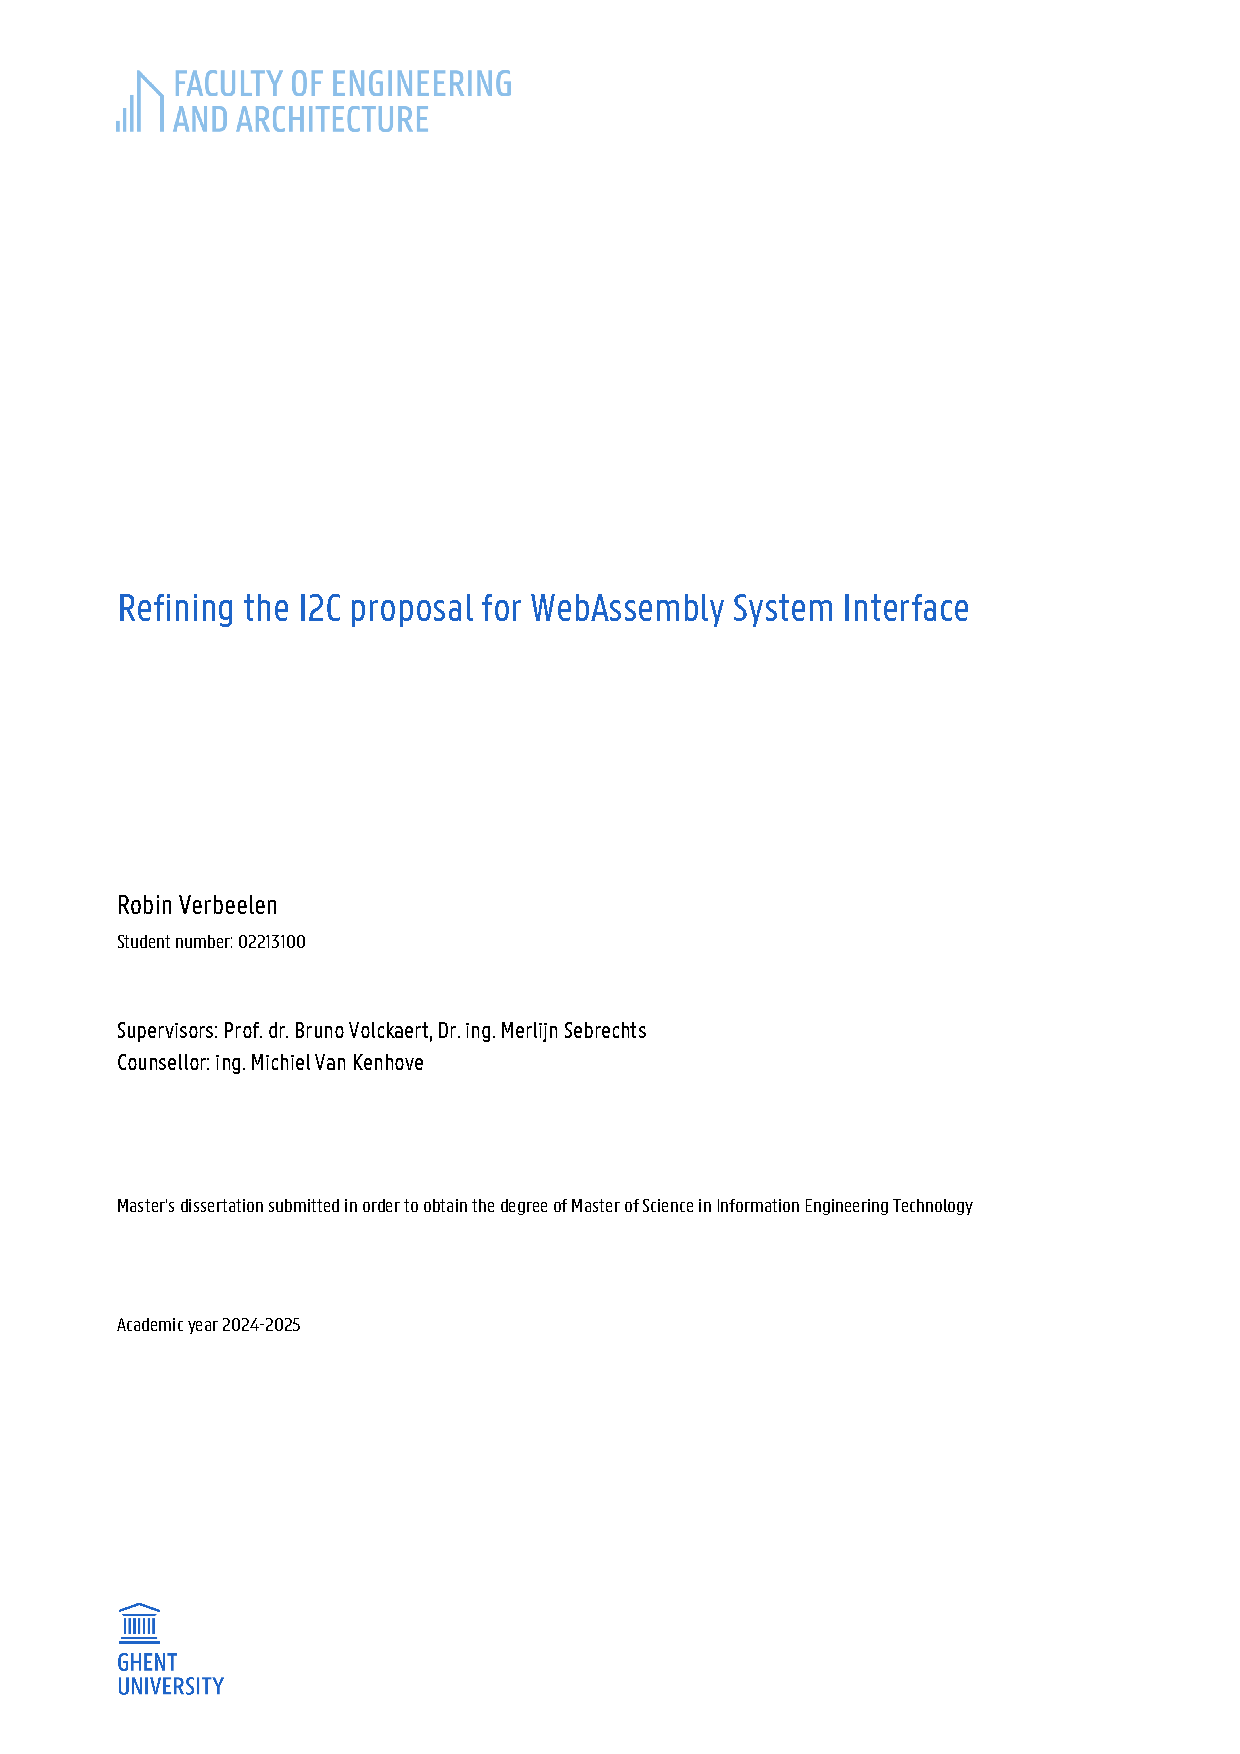
\includepdf{cover-sheet.pdf}

% Only add this Chapter if applicable
\chapter*{Statement of confidentiality}

Confidential up to and including dd/mm/yyyy

Important

This master’s dissertation contains confidential information and/or confidential research results proprietary to Ghent University or third parties. It is strictly forbidden to publish, cite or make public in any way this master’s dissertation or any part thereof without the express written permission of Ghent University. Under no circumstance may this master’s dissertation be communicated to or put at the disposal of third parties. Photocopying or duplicating it in any other way is strictly prohibited. Disregarding the confidential nature of this master’s dissertation may cause irremediable damage to Ghent University. The stipulations mentioned above are in force until the embargo date.
\chapter*{Acknowledgment}
\addcontentsline{toc}{chapter}{Acknowledgments}

I would like to express my sincere gratitude to all those who contributed to the successful completion of this master's thesis.

First and foremost, I extend my heartfelt thanks to my promotors, Prof. Dr. Bruno Volckaert and Dr. Merlijn Sebrechts, for placing their trust in me and providing the opportunity to participate in this research. Your confidence in my abilities has been invaluable throughout this journey.

Later in the year, Friedrich Vandenberghe, MSc in Industrial Engineering, joined our team as my predecessor on this thesis topic. Friedrich, your extensive experience with this research theme and your valuable contributions from the middle phase of my trajectory on have significantly enriched my work. Your insights and willingness to share your knowledge have been tremendously helpful.

I want to especially acknowledge Merlijn, Michiel, and Friedrich together again for always being available whenever I wanted to discuss results, share ideas, or seek advice. Your open-door policy and genuine interest in my progress have made this research journey both productive and enjoyable.

Finally, I would like to thank my girlfriend, friends, and parents for their unwavering support and genuine interest in my research. Your encouragement and curiosity about my work provided the extra motivation I needed to strive for excellent results. Your belief in me has been a constant source of strength throughout this challenging but rewarding experience.

This thesis would not have been possible without the collective support, guidance, and encouragement of all the individuals mentioned above. Thank you for making this journey memorable and successful.
\chapter*{Explanation regarding the master's thesis and the oral presentation}


This master's dissertation is part of an exam. Any comments formulated by the assessment committee during the oral presentation of the master's dissertation are not included in this text.

%%%%%%%%%%%%%%%%%%%%%%%%%%%%%%
%    Dutch version           %
%%%%%%%%%%%%%%%%%%%%%%%%%%%%%%
%
% \chapter*{Toelichting in verband met het masterproefwerk}
%
% Deze masterproef vormt een onderdeel van een examen. Eventuele opmerkingen die door de beoordelingscommissie tijdens de mondelinge uiteenzetting van de masterproef werden geformuleerd, werden niet verwerkt in deze tekst.
\chapter*{Abstract}
\chaptermark{Abstract}
\addcontentsline{toc}{chapter}{Abstract}  

This chapter should contain three things.

\begin{itemize}
    \item A copy of all the information on the title page of your master's thesis. This includes things like the name of your master's thesis and your advisors.
    \item A one-paragraph description of your master's thesis. This should be 15 to 20 lines long. This should include the context of your master's thesis, the problem statement of your master's thesis. The results of your master's thesis, and the evaluation of the work.
    \item Five keywords that describe the subject best.
\end{itemize}

The chapter should be one page at most.

% How to add the extended abstract:
%
% You should write the extended abstract as a separate overleaf project. Then compile it there, download the PDF, and upload it to this project.
%
% Use the "IEEE conference proceedings template" to create the extended abstract project. 
% https://www.overleaf.com/latex/templates/ieee-conference-template/grfzhhncsfqn
%
% Then download the final PDF, upload it to the root of this project, and point the statement below to the correct file.
\phantomsection
\addcontentsline{toc}{chapter}{Extended Abstract}
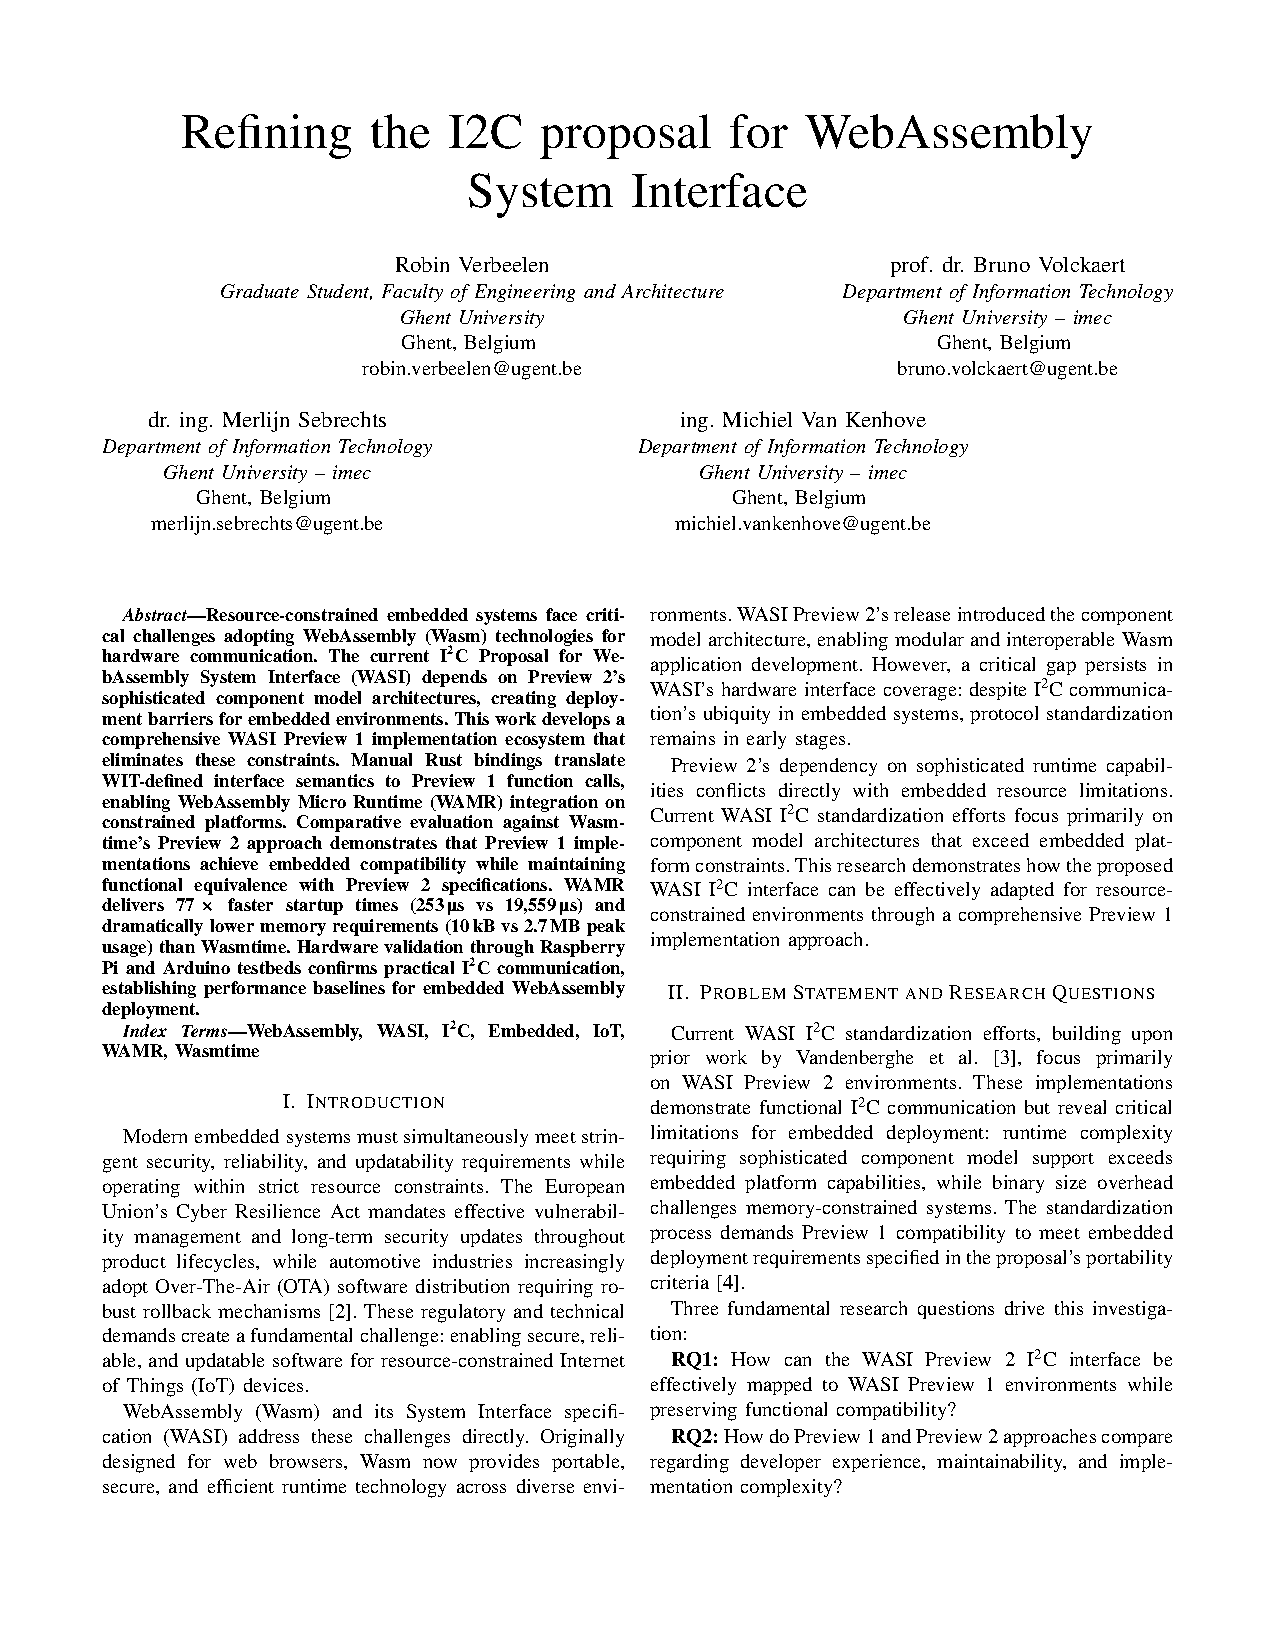
\includepdf[pages={-}]{extended-abstract.pdf}
\tableofcontents\newpage
\listoffigures\newpage
\listoftables\newpage
\printglossary[type=\acronymtype, title={List of Acronyms}]

\glsaddallunused[\acronymtype]                              % make sure all unused acronyms are in list

\setlist[description]{style=standard} % reset list settings back to default

\listoflistings\newpage

%
% Include the main chapters of the thesis below
% Note: it's best to avoid spaces in filenames as Latex might complain about them.
%
\mainmatter
\pagestyle{fancy} % Use header
\chapter{Introduction}
\label{chap:intro}

\textit{Note: in most master's theses, the Introduction is a full-blow introductory chapter. That's why this chapter is numbered.}

This template supports Unicode natively so special characters like ``é'' and ``ë'' work by default.

As is visible in Figure~\ref{fig:cloud_rollen}, the cloud provider manages the IaaS and PaaS stacks.

\begin{figure}[h]
	\centering
	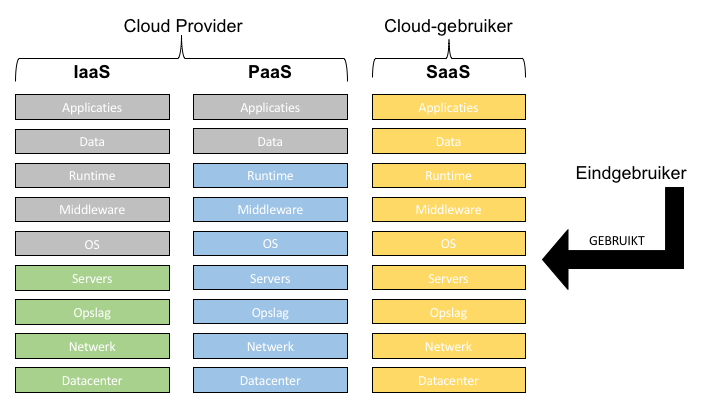
\includegraphics[width=\textwidth]{images/cloud_rollen.png}
	\caption{Image with caption.}
	\label{fig:cloud_rollen}
\end{figure}

Example of a code fragment. Minted supports modern programming languages such as Rust and Golang, and modern configuration formats such as YAML.

\begin{listing}[ht]
\begin{minted}[fontsize=\footnotesize,samepage]{rs}
// This is the main function.
fn main() {
    // Statements here are executed when the compiled binary is called.

    // Print text to the console.
    println!("Hello World!");
}
\end{minted}
\caption{This hello-world code fragment is deceivingly simple. Most rust programs are a lot more difficult to comprehend.}
\end{listing}



\section{Section title}

Table~\ref{tab:resallocschemes} shows an overview of..

\begin{table}[h]
	\centering
	\captionsetup{justification=centering}
	\caption[Overzicht resource-allocatieschema's]{Overzicht resource-allocatieschema's}
	\label{tab:resallocschemes}
	\resizebox{\textwidth}{!}{%
	\begin{tabular}{L{4cm} l C{2cm} c c c c}
		\toprule
		Naam & Jaar & Type  & A | F | P  & Invoer & Uitvoer & Getest  \\ \midrule
		Alicherry et al.~\cite{Alicherry2012} & 2012 & k-sneden & A & G & par\{G\} & S \\
		MCRVMP~\cite{Biran2012} & 2012 & ILP \& GH & A & B\{netwerk\} & VM-plaatsing & C\\
		\bottomrule
	\end{tabular}}
\end{table}

\include{chapters/8_chapter_1.tex}
\chapter{Title of the second chapter}
\label{chap:1}

Text of the second chapter

\section{Section title 1}
\label{sec:1}

Text.

\section{Section title 2}

Text.

\chapter{Title of the third chapter}
\label{chap:2}

Text of the third chapter

\chapter{Performance Analysis}
\label{chap:performance-analysis}

\section{Introduction}
\label{sec:perf-intro}

% TODO: Write brief intro explaining:
% - Purpose of performance evaluation 
% - Focus on WAMR vs Wasmtime comparison
% - Native as baseline reference
% - Overview of what will be analyzed (timing, memory, correctness)

\section{Experimental Setup}
\label{sec:experimental-setup}

\subsection{Hardware Configuration}
\label{subsec:hardware-config}

% TODO: Describe your Pi + Arduino setup
% - Raspberry Pi specifications (model, OS, architecture)
% - Arduino Uno specifications
% - I2C connection between Pi and Arduino
% - Physical wiring diagram (reference to figure if you make one)
% - Why Arduino was chosen for I2C communication

The experimental setup consists of a Raspberry Pi connected to an Arduino Uno via I2C communication.

\textbf{Raspberry Pi Configuration:}
% TODO: Fill in your specific Pi details
\begin{itemize}
    \item Model: YOUR\_PI\_MODEL
    \item Architecture: aarch64-unknown-linux-musl
    \item Operating System: YOUR\_OS\_VERSION
    \item I2C Interface: Hardware I2C via GPIO pins SPECIFY\_PINS
\end{itemize}

\textbf{Arduino Uno Configuration:}
% TODO: Fill in Arduino details
\begin{itemize}
    \item Model: Arduino Uno
    \item I2C Address: [YOUR\_I2C\_ADDRESS] 
    \item Serial Monitor: Used for correctness verification
    \item Firmware: [DESCRIBE\_YOUR\_ARDUINO\_CODE\_BRIEFLY]
\end{itemize}

% TODO: Add figure of your hardware setup if you have photos
% \begin{figure}[htbp]
% \centering
% \includegraphics[width=0.8\textwidth]{figures/hardware-setup}
% \caption{Raspberry Pi and Arduino I2C Test Setup}
% \label{fig:hardware-setup}
% \end{figure}

\subsection{Benchmark Methodology}
\label{subsec:benchmark-methodology}

The performance evaluation follows a two-stage approach to ensure both correctness and reliable performance measurements.

\subsubsection{Stage 1: Correctness Verification}

% TODO: Explain your correctness verification process
Before conducting performance measurements, correctness verification is performed:
\begin{enumerate}
    \item [DESCRIBE\_VERIFICATION\_PROCESS]
    \item Arduino serial monitor output verification
    \item [WHAT\_DO\_YOU\_CHECK\_SPECIFICALLY?]
    \item [HOW\_DO\_YOU\_VERIFY\_READ/WRITE\_SUCCESS?]
\end{enumerate}

% TODO: Maybe include example serial output or reference to appendix
% \begin{lstlisting}[caption=Example Arduino Serial Output for Verification,label=lst:serial-output]
% // TODO: Include actual serial output from your Arduino
% // showing successful I2C communication
% \end{lstlisting}

\subsubsection{Stage 2: Performance Measurement}

% TODO: Describe your Criterion benchmark setup
After correctness verification, performance measurements are conducted using:
\begin{itemize}
    \item \textbf{Framework:} Criterion.rs statistical benchmarking
    \item \textbf{Output Format:} JSON for automated analysis
    \item \textbf{Measurement Types:} [LIST\_YOUR\_BENCHMARK\_CATEGORIES]
    \item \textbf{Statistical Method:} [DESCRIBE\_CRITERION\_SETTINGS]
\end{itemize}

The ``ping-pong'' operation consists of:
% TODO: Describe your exact ping-pong implementation
\begin{enumerate}
    \item Write [X] bytes to I2C address [ADDRESS]: \texttt{[YOUR\_DATA\_BYTES]}
    \item Read [X] bytes from the same I2C address
    \item [ANY\_VERIFICATION\_STEP?]
\end{enumerate}

\section{Performance Results}
\label{sec:performance-results}

\subsection{Runtime Setup Performance}
\label{subsec:setup-performance}

% TODO: Present your setup timing results
Table~\ref{tab:setup-performance} shows the initialization time for each runtime implementation.

\begin{table}[htbp]
\centering
\caption{Runtime Setup Performance Comparison}
\label{tab:setup-performance}
\begin{tabular}{lrrr}
\toprule
\textbf{Implementation} & \textbf{Mean (ns)} & \textbf{Std Dev (ns)} & \textbf{Relative to Native} \\
\midrule
% TODO: Fill in your actual benchmark results
Native        & [FILL\_NATIVE\_SETUP]    & [FILL\_STD]  & 1.0x \\
WAMR          & [FILL\_WAMR\_SETUP]      & [FILL\_STD]  & [CALC]x \\
Wasmtime      & [FILL\_WASMTIME\_SETUP]  & [FILL\_STD]  & [CALC]x \\
\bottomrule
\end{tabular}
\end{table}

% TODO: Add your analysis of setup performance
% Focus on WAMR vs Wasmtime differences
% Why is Wasmtime so much slower?
% Implications for embedded usage

\subsection{Execution Performance}
\label{subsec:execution-performance}

\subsubsection{Cold Execution}

% TODO: Present cold execution results
Table~\ref{tab:cold-performance} presents the performance of the first execution after runtime setup.

\begin{table}[htbp]
\centering
\caption{Cold Execution Performance}
\label{tab:cold-performance}
\begin{tabular}{lrrr}
\toprule
\textbf{Implementation} & \textbf{Mean (ns)} & \textbf{95\% CI Lower} & \textbf{95\% CI Upper} \\
\midrule
% TODO: Fill in your cold execution data
Native        & [FILL]    & [FILL]  & [FILL] \\
WAMR          & [FILL]    & [FILL]  & [FILL] \\
Wasmtime      & [FILL]    & [FILL]  & [FILL] \\
\bottomrule
\end{tabular}
\end{table}

\subsubsection{Hot Execution}

% TODO: Present hot execution results
Table~\ref{tab:hot-performance} shows steady-state performance after runtime warmup.

\begin{table}[htbp]
\centering
\caption{Hot Execution Performance}
\label{tab:hot-performance}
\begin{tabular}{lrrr}
\toprule
\textbf{Implementation} & \textbf{Mean (ns)} & \textbf{Median (ns)} & \textbf{MAD (ns)} \\
\midrule
% TODO: Fill in your hot execution data
Native        & [FILL]    & [FILL]  & [FILL] \\
WAMR          & [FILL]    & [FILL]  & [FILL] \\
Wasmtime      & [FILL]    & [FILL]  & [FILL] \\
\bottomrule
\end{tabular}
\end{table}

% TODO: Add performance comparison figure
% \begin{figure}[htbp]
% \centering
% \includegraphics[width=0.9\textwidth]{figures/execution-performance-comparison}
% \caption{Execution Performance Comparison: WAMR vs Wasmtime vs Native}
% \label{fig:execution-comparison}
% \end{figure}

\section{Statistical Analysis}
\label{sec:statistical-analysis}

% TODO: Add statistical analysis of your results
\subsection{Significance Testing}

% TODO: Perform and report statistical tests
% Mann-Whitney U test between WAMR and Wasmtime
% Effect size calculations
% Discussion of practical vs statistical significance

\subsection{Performance Variability}

% TODO: Analyze the stability/consistency of your measurements
% Compare variability between implementations
% Discuss implications for real-world usage

% TODO: Reference box plots or violin plots showing distribution
% \begin{figure}[htbp]
% \centering
% \includegraphics[width=0.9\textwidth]{figures/performance-distributions}
% \caption{Performance Distribution Comparison}
% \label{fig:performance-distributions}
% \end{figure}

\section{Memory Usage Analysis}
\label{sec:memory-analysis}

\subsection{DHAT Profiling Setup}

% TODO: Explain your DHAT configuration
Memory profiling was conducted using DHAT (Dynamic Heap Analysis Tool) with the following configuration:
\begin{itemize}
    \item \textbf{Profiling Targets:} [SPECIFY\_WHAT\_YOU\_PROFILED]
    \item \textbf{Measurement Phases:} Runtime setup, ping-pong execution
    \item \textbf{Output Format:} JSON for automated analysis
\end{itemize}

\subsection{Runtime Setup Memory Usage}

% TODO: Present DHAT results for setup phase
Table~\ref{tab:memory-setup} shows memory allocation patterns during runtime initialization.

\begin{table}[htbp]
\centering
\caption{Memory Usage During Runtime Setup}
\label{tab:memory-setup}
\begin{tabular}{lrrr}
\toprule
\textbf{Implementation} & \textbf{Peak Heap (KB)} & \textbf{Total Allocs} & \textbf{Avg Alloc Size (B)} \\
\midrule
% TODO: Fill in your DHAT setup results
Native        & [FILL]    & [FILL]  & [FILL] \\
WAMR          & [FILL]    & [FILL]  & [FILL] \\
Wasmtime      & [FILL]    & [FILL]  & [FILL] \\
\bottomrule
\end{tabular}
\end{table}

\subsection{Execution Memory Usage}

% TODO: Present DHAT results for ping-pong execution
Table~\ref{tab:memory-execution} shows memory usage patterns during ping-pong operations.

\begin{table}[htbp]
\centering
\caption{Memory Usage During Ping-Pong Execution}
\label{tab:memory-execution}
\begin{tabular}{lrrr}
\toprule
\textbf{Implementation} & \textbf{Heap Growth (KB)} & \textbf{Execution Allocs} & \textbf{Memory Lifetime (ms)} \\
\midrule
% TODO: Fill in your DHAT execution results
Native        & [FILL]    & [FILL]  & [FILL] \\
WAMR          & [FILL]    & [FILL]  & [FILL] \\
Wasmtime      & [FILL]    & [FILL]  & [FILL] \\
\bottomrule
\end{tabular}
\end{table}

% TODO: Analyze memory usage differences
% Why does Wasmtime use more memory?
% Implications for embedded systems
% Memory efficiency comparison

\section{WAMR vs Wasmtime Comparison}
\label{sec:wamr-vs-wasmtime}

% TODO: This is your main focus section
% Direct comparison of the two WebAssembly runtimes
% Analyze strengths/weaknesses of each approach

\subsection{Performance Characteristics}

% TODO: Compare performance profiles
\begin{itemize}
    \item \textbf{Setup Performance:} [ANALYZE\_SETUP\_DIFFERENCES]
    \item \textbf{Steady-State Performance:} [ANALYZE\_EXECUTION\_DIFFERENCES] 
    \item \textbf{Memory Efficiency:} [COMPARE\_MEMORY\_USAGE]
    \item \textbf{Performance Consistency:} [COMPARE\_VARIABILITY]
\end{itemize}

\subsection{Architecture Differences}

% TODO: Discuss architectural differences affecting performance
\begin{itemize}
    \item \textbf{WASI Preview 1 vs Preview 2:} [IMPACT\_ON\_PERFORMANCE]
    \item \textbf{Component Model Overhead:} [WASMTIME\_SPECIFIC\_COSTS]
    \item \textbf{Handwritten vs Generated Bindings:} [BINDING\_IMPACT]
    \item \textbf{Runtime Optimizations:} [DIFFERENT\_OPTIMIZATION\_STRATEGIES]
\end{itemize}

\subsection{Embedded Suitability}

% TODO: Evaluate suitability for embedded applications
\begin{itemize}
    \item \textbf{Resource Constraints:} [MEMORY\_CPU\_REQUIREMENTS]
    \item \textbf{Startup Latency:} [IMPACT\_ON\_REAL\_APPLICATIONS]
    \item \textbf{Deterministic Performance:} [REAL\_TIME\_CONSIDERATIONS]
    \item \textbf{Development Experience:} [TOOLING\_DEBUGGING\_SUPPORT]
\end{itemize}

\section{Flame Graph Analysis}
\label{sec:flamegraph-analysis}

% TODO: Analyze your pprof flame graph results
Flame graph analysis provides insights into CPU time distribution during execution.

% TODO: Reference your flame graph figure
% \begin{figure}[htbp]
% \centering
% \includegraphics[width=1.0\textwidth]{figures/flamegraph-comparison}
% \caption{CPU Time Distribution Flame Graph}
% \label{fig:flamegraph}
% \end{figure}

% TODO: Analyze what the flame graph shows
% Where is time spent in each implementation?
% What are the bottlenecks?
% How do call stacks compare between WAMR and Wasmtime?

\subsection{Hotspot Analysis}

% TODO: Identify performance hotspots from flame graph
\begin{itemize}
    \item \textbf{WAMR Hotspots:} [IDENTIFY\_EXPENSIVE\_FUNCTIONS]
    \item \textbf{Wasmtime Hotspots:} [IDENTIFY\_EXPENSIVE\_FUNCTIONS]
    \item \textbf{Common Bottlenecks:} [SHARED\_EXPENSIVE\_OPERATIONS]
\end{itemize}

\subsection{Call Stack Comparison}

% TODO: Compare call stack depth and complexity
% Which runtime has simpler/more complex execution paths?

\section{Summary}
\label{sec:performance-summary}

% TODO: Brief summary of key findings
% Keep this short since you'll have full conclusion chapter
This chapter presented a comprehensive performance analysis comparing WAMR and Wasmtime implementations of the I2C WASI interface.

\textbf{Key Findings:}
\begin{itemize}
    \item [SUMMARIZE\_SETUP\_PERFORMANCE\_DIFFERENCE]
    \item [SUMMARIZE\_EXECUTION\_PERFORMANCE\_SIMILARITY]
    \item [SUMMARIZE\_MEMORY\_USAGE\_DIFFERENCES] 
    \item [SUMMARIZE\_EMBEDDED\_SUITABILITY\_ASSESSMENT]
\end{itemize}

% TODO: Lead into next chapter (Discussion?)
The implications of these findings for embedded WebAssembly applications are discussed in Chapter~\ref{chap:discussion}.
\include{chapters/8_chapter_5.tex}
\chapter*{Conclusion}
\chaptermark{Conclusion}
\addcontentsline{toc}{chapter}{Conclusion}  

Fill in..

\chapter*{Future Work}
\chaptermark{Future Work}
\addcontentsline{toc}{chapter}{Future Work}  

This chapter explains what the next steps are to continue the research and innovation of your master's thesis. Are there any additional features of research directions that are interesting? Are there ways in which your solution can be improved?

\chapter*{Societal Reflection}
\chaptermark{Societal Reflection}
\addcontentsline{toc}{chapter}{Societal Reflection}

% TODO: Duurzaamheidsreflectie kan bespreken dat het gebruik van wasm oudere hardware terug leven kan geven omdat deze techniek minder kost resources nodig heeft dan andere virtualisatie methoden. Maar uitgebreid onderzoek doen naar resultaten van andere onderzoeken die aanwijzen hoeveel dedicated virtualisatietechnieken voor embedded/contraint devices inhoudt.

This chapter is only for the engineering technology ("industrieel ingenieur") students. It contains a societal reflection of one to three pages. You can interpret this very broadly. For example, this chapter can include one or more of the following.

\begin{itemize}
    \item Placing the work in a broader societal context. For example, how does this work impact or contribute to recent societal change such as digital transformation or the AI revolution?
    \item Explaining how the work contributes to the implementation of the United Nations (UN) Sustainable Development Goals (SDGs). For more information, see \url{https://en.wikipedia.org/wiki/Sustainable_Development_Goals} and \url{https://www.sdgs.be/nl/sdgs}.
    \item Reflecting on the ethical impact of this thesis or the used datasets. For example, how does this impact people's privacy? Is there bias available in the datasets? Could this be used for military or dual-use purposes?
    \item Investigating how the resulting work conforms to relevant laws or technical standards such as the GDPR, AI act and the CRA.
\end{itemize}

\renewcommand\bibname{References}
\bibliography{references.bib}

%%%%%%%%%%%%%%%%%%%%%%%%%%%%%%
%    Dutch version           %
%%%%%%%%%%%%%%%%%%%%%%%%%%%%%%
% \renewcommand\bibname{Referenties}
% \bibliography{references.bib}

\begin{appendices}
\section*{Attachment A}
\addcontentsline{toc}{section}{Attachment A}  

Attachment description.



\newpage
\section*{Attachment B}
\addcontentsline{toc}{section}{Attachment B}  

Attachment description.

\end{appendices}

%%%%%%%%%%%%%%%%%%%%%%%%%%%%%%
%    Dutch version           %
%%%%%%%%%%%%%%%%%%%%%%%%%%%%%%
% \begin{appendices}
% \section*{Bijlage A}
% \addcontentsline{toc}{section}{Bijlage A}  

% Toelichting bijlage.



% \newpage
% \section*{Bijlage B}
% \addcontentsline{toc}{section}{Bijlage B}  

% Toelichting bijlage.

% \end{appendices}


\pagestyle{numberless} 
\pagestyle{empty}
\begin{appendices}
\section*{Attachment A}
\addcontentsline{toc}{section}{Attachment A}  

Attachment description.



\newpage
\section*{Attachment B}
\addcontentsline{toc}{section}{Attachment B}  

Attachment description.

\end{appendices}

%%%%%%%%%%%%%%%%%%%%%%%%%%%%%%
%    Dutch version           %
%%%%%%%%%%%%%%%%%%%%%%%%%%%%%%
% \begin{appendices}
% \section*{Bijlage A}
% \addcontentsline{toc}{section}{Bijlage A}  

% Toelichting bijlage.



% \newpage
% \section*{Bijlage B}
% \addcontentsline{toc}{section}{Bijlage B}  

% Toelichting bijlage.

% \end{appendices}


\end{document}
